\documentclass[11pt,a4paper]{article}

\usepackage[review]{acl}
\usepackage{booktabs}
\usepackage{graphicx}
\usepackage{microtype}
\usepackage{amsmath}
\usepackage{url}
\usepackage{fontspec}
\usepackage{polyglossia}
\setdefaultlanguage{english}
\setotherlanguage{arabic}
\newfontfamily\arabicfont[Script=Arabic]{Amiri}

\title{Natural, Synthetic, or Mixed Supervision for Open-Weight Arabic
Grammatical Error Correction}

\author{Anonymous ACL submission}

\begin{document}
\maketitle

\begin{abstract}
Modern Standard Arabic grammatical error correction (GEC) remains
underexplored for open-weight instruction-tuned large language models (LLMs).
We study how natural, synthetic, and mixed supervision affect a practical
highlighted-token correction task while holding the model, training-set size,
and evaluation protocol fixed.  We fine-tune Gemma 3 4B with QLoRA on three
equal 2,000-record views and evaluate once on 511 Nahw-Passage records.  Mixed
supervision reaches 31.70\% exact-match accuracy, compared with 20.55\% for
synthetic-only and 28.38\% for natural-only; the mixed--natural difference is
not established.  Post-hoc robustness analyses preserve the mixed-over-
synthetic direction.  Auxiliary diagnostics reveal a trade-off: synthetic-
only changes fewer already-correct tokens, whereas mixed supervision retains
more ArabicMMLU capability.  These findings show that supervision composition
materially affects open-weight Arabic GEC, while one model and strict single-
reference scoring limit generality.
\end{abstract}

\section{Introduction}

Grammatical error correction requires a model to produce a valid correction,
not merely recognize a grammatical rule.  This distinction is consequential
for Modern Standard Arabic (MSA), whose rich morphology and agreement systems
create substantial correction ambiguity.  Arabic GEC research has benefited
from the QALB shared tasks \citep{mohit-etal-2014-first,
rozovskaya-etal-2015-second}, specialized sequence-to-sequence systems
\citep{nagoudi-etal-2022-arat5,alhafni-etal-2023-advancements}, and recent
prompting and instruction-tuning studies \citep{kwon-etal-2023-beyond}.
Nevertheless, the effect of \emph{supervision source} is difficult to isolate
when model families, corpus sizes, tasks, and evaluation protocols vary
together.

Nahw provides a recent benchmark spanning Arabic grammar understanding, error
detection, correction, and explanation \citep{mubarak-etal-2026-nahw}.  Its
fine-tuning study focuses on grammar understanding, leaving direct
fine-tuning for its practical correction task open.  We address that gap with
a controlled extension to highlighted-token correction.  Using one fixed
Gemma 3 4B instruction-tuned LLM revision \citep{gemma-team-2025-gemma3}, we
compare equal-size
natural-only, synthetic-only, and mixed training views while holding the
training and evaluation interfaces fixed.

Our primary question is whether a fixed natural--synthetic mixture improves
over size-matched synthetic-only supervision.  We specify and freeze this
comparison before either adapter accesses Nahw-Passage, retain row-level outputs
privately, and reproduce the paired statistics from aligned predictions.  We
also report the earlier natural-only result and later prompt-only baselines as
explicitly staged comparisons rather than presenting all five systems as one
simultaneous experiment.

The study is intentionally a controlled case study rather than a new model
architecture.  Its central contribution is to isolate supervision composition
under one task and one open-weight LLM.  This design strengthens the internal
comparison, while necessarily limiting claims about other model families,
scales, or Arabic correction settings.

Our contributions are:
\begin{itemize}
    \item a controlled GEC fine-tuning extension of Nahw using an open-weight
    instruction-tuned LLM;
    \item an equal-record comparison of natural, released-synthetic, and fixed
    mixed supervision with deterministic data selection and overlap controls;
    \item a frozen 511-record paired evaluation showing a large mixed-over-
    synthetic-only advantage;
    \item a post-hoc five-seed cohort in which the mixed arm exceeds the
    synthetic-only arm under dev-selected and matched fixed checkpoints; and
    \item an auditable, privacy-conscious protocol that records exact model,
    data, checkpoint, decoding, and artifact identities without publishing
    restricted corpus text or model responses.
\end{itemize}

\section{Related Work}

\paragraph{Arabic GEC.}
The QALB 2014 and 2015 shared tasks established standard Arabic text
correction datasets and evaluation procedures
\citep{mohit-etal-2014-first,rozovskaya-etal-2015-second}.  Later work improved
Arabic grammatical error detection and correction through pretrained Arabic
models, morphology-aware components, and multitask learning
\citep{alhafni-etal-2023-advancements}.  AraT5 demonstrated the utility of
Arabic-focused text-to-text pretraining for generation tasks, including GEC
\citep{nagoudi-etal-2022-arat5}.

Recent Arabic text-editing work derives language-independent edit tags from
training data, improving both correction quality and decoding efficiency
\citep{alhafni-habash-2025-enhancing}.  That work advances the editing
formulation.  Our question is complementary: with one model revision,
fine-tuning recipe, record count, task interface, and evaluation fixed, how
does the source composition of supervision affect correction?

\citet{kwon-etal-2023-beyond} compare prompted instruction-following models
with fully fine-tuned Arabic GEC systems and explore synthetic augmentation.
Their results motivate both prompt-only baselines and synthetic supervision.
On QALB-2014, they report M2 $F_{0.5}$ scores of 67.82 for five-shot GPT-4,
70.81 for an AraT5v2 baseline, and 75.27 after large-scale synthetic
augmentation.  These full-sentence edit scores are not numerically comparable
to our token-level exact-match measure.  Their systems also differ in
architecture, training scale, and data source, so they do not provide a
matched contrast between natural, synthetic, and mixed data.

More broadly, synthetic GEC data can be valuable but is not automatically
equivalent to human-annotated supervision.  Prior work identifies mismatched
error distributions and noisy labels as obstacles to using synthetic data in
data-limited fine-tuning, and improves results through contextual generation
and relabeling \citep{wang-etal-2024-improving-grammatical}.  This motivates
testing composition directly rather than treating all training pairs as
exchangeable.

\paragraph{Arabic grammar benchmarks and synthetic data.}
Nahw evaluates grammar understanding, detection, correction, and explanation
and finds substantial weaknesses across current models
\citep{mubarak-etal-2026-nahw}.  The 511-error Nahw-Passage component supports
highlighted-token correction, which is narrower than full-sentence QALB
correction but permits tightly aligned paired evaluation.

Tibyan is a released synthetic Arabic GEC corpus created with
ChatGPT-assisted generation and iterative linguistic review
\citep{alrehili-alhothali-2024-tibyan}.  Its release contains sentence pairs
but no official split, stable identifiers, or record-level error labels.
ARETA provides automatic Arabic error categories
\citep{belkebir-habash-2021-automatic}, but automatic labels are not expert
gold.  We therefore derive a deterministic highlighted-token view without
assigning linguistic error types.

\section{Datasets and Experimental Controls}

\begin{table*}[t]
\centering
\scriptsize
\setlength{\tabcolsep}{4pt}
\begin{tabular}{p{2.2cm}p{3.0cm}p{2.6cm}p{6.9cm}}
\toprule
Dataset & Source & Released size & Use in this study \\
\midrule
QALB 2014 L1 & \citet{mohit-etal-2014-first} & 19,411 train; 1,017 dev; 968 test & 2,000 filtered train records for F1; the nested first 1,000 for F3; 975 filtered dev records for checkpoint selection. Test is unused. \\
Tibyan & \citet{alrehili-alhothali-2024-tibyan} & 6,192 sentence pairs & Deterministic highlighted-token conversion; 2,000 project-train records for F2; the nested first 1,000 for F3. \\
Nahw-Passage & \citet{mubarak-etal-2026-nahw} & 100 passages, 511 correction records & All 511 records form the single frozen final test; never used for training, prompting, or selection. \\
QALB 2015 L2 dev & \citet{rozovskaya-etal-2015-second} & 154 records & Reconstructed corrected targets for the matched already-correct-token diagnostic. \\
ArabicMMLU & \citet{koto-etal-2024-arabicmmlu} & 14,575 questions, 40 tasks & Fixed balanced 1,000-question auxiliary capability diagnostic (25 per task). \\
\bottomrule
\end{tabular}
\caption{Datasets, release sizes, and experimental roles. Restricted corpus
text is not reproduced.}
\label{tab:datasets}
\end{table*}

\subsection{Task and final evaluation}

Each example supplies an MSA passage and one highlighted erroneous token.  The
model must return only the corrected token.  We use all 511 ordered
Nahw-Passage correction records as a test-only set.

\noindent\textbf{Illustrative task example (author-created; not corpus text).}
Passage: \textarabic{هؤلاء الطالب يكتبون الدرس.}  Highlighted token:
\textarabic{الطالب}.  Required output: \textarabic{الطلاب}.  English:
``These students write the lesson.''  The model receives the passage and
highlighted token but must output only the replacement token, not a rewritten
sentence or explanation.

Our primary metric is \emph{exact-match accuracy (EM)}: the percentage of
records for which the frozen parser's predicted token exactly equals the
single reference after permitted outer-format and whitespace removal.  We
apply no Arabic-letter, hamza, diacritic, or spelling normalization.  Thus a
linguistically plausible alternative receives no credit if it differs from
the reference.  We use ``exact-match accuracy'' consistently for this task;
ArabicMMLU uses conventional multiple-choice accuracy.

Nahw-Passage is never used for training, prompt design, checkpoint
selection, or development generation.  The frozen prepared input identity is
recorded in the public audit; all evaluated systems use the same
ordered records.

\subsection{Natural supervision}

The natural view is derived from QALB 2014 L1 training data
\citep{mohit-etal-2014-first}.  We retain annotator-0 actions that replace
exactly one source token with one nonempty correction token, require the
erroneous token to occur once, and retain at most one eligible action per
document.  A content-neutral SHA-256 ordering with seed 3407 selects 2,000
records.  QALB development and test records are excluded.  We use a separately
selected 975-record QALB 2014 L1 development view only for assistant-token
loss and technical validation.  QALB test is not used for training,
development, prompting, or evaluation.

\subsection{Synthetic and mixed supervision}

Tibyan releases 6,192 erroneous--corrected sentence pairs under CC BY 4.0
\citep{alrehili-alhothali-2024-tibyan}.  Because a strict whole-pair
single-substitution filter retains only three pairs, we compute minimum-edit
alignments and retain a substitution only when it is forced across every
optimal alignment.  We require one occurrence of the erroneous token, create
connected groups for repeated exact sides, and retain at most one seeded
representative per group.  This yields 6,165 candidate pairs in 6,156 groups.

Tibyan has no official train/development split.  We assign groups to an
80:20 project split by seeded SHA-256 buckets.  Before splitting, exact
UTF-8 hashes of both sides are compared with all registered QALB splits and
with Nahw fields; any matching group would be excluded.  This check finds no
exact full-side overlap, although it cannot detect paraphrases or pretraining
contamination.

The synthetic arm (\textbf{F2}) takes the first 2,000 eligible project-training
representatives under a fixed hash order.  The mixed arm (\textbf{F3}) combines
the first 1,000 records in the frozen natural order with the first 1,000 in the
frozen synthetic order.  Thus both halves are nested subsets of their
single-source arms rather than new samples.  The natural arm (\textbf{F1}),
F2, and F3 each contain exactly 2,000 records.

\section{Systems and Training}

\subsection{Model choice}

We use Gemma 3 4B because it is an open-weight, multilingual,
instruction-tuned LLM that supports the Arabic task interface while remaining
small enough for 4-bit QLoRA on a free 16~GB P100.  Fixing one public revision
also makes supervision composition the principal controlled variable and keeps
all three trainable arms computationally feasible.  This practical choice is
not evidence that Gemma is uniquely suitable for Arabic GEC; dependence on one
model and scale limits external validity.

\subsection{Prompt-only baselines}

Both baselines use the untouched 4-bit Gemma 3 4B instruction-tuned LLM at the
same fixed revision.  \textbf{B1} prepends five QALB-training demonstrations
selected by a content-neutral hash rule.  Its Arabic query then says, in
English translation: ``Correct the specified erroneous word in the following
text. Return only the corrected word, without explanation or quotation
marks.''  The exact query is \textarabic{صحح الكلمة الخاطئة المحددة في النص
التالي. أعد الكلمة المصححة فقط دون شرح أو علامات اقتباس.}  \textbf{B2} uses no
demonstrations and asks an Arabic-correction tool
to determine the correct form from context, leave the rest unchanged, and
return only that word: \textarabic{أنت أداة متخصصة في تصحيح العربية الفصحى.
راجع سياق النص لتحديد الصيغة الصحيحة للكلمة المحددة، مع إبقاء بقية النص دون
تغيير. أعد الكلمة المصححة فقط دون شرح أو تعليل أو علامات اقتباس.}  The exact
Arabic templates are public in the code;
restricted demonstration and passage text is not reproduced.  ``Expert-style''
names the prompt design, not expert validation.

\subsection{QLoRA fine-tuning}

We train fresh unmerged adapters with QLoRA
\citep{dettmers-etal-2023-qlora}.  The 4-bit base, processor, Arabic task
instruction, response-only objective, and maximum formatted length of 1,024
tokens are shared.  LoRA uses rank 16, alpha 32, zero dropout, no bias, and the
query, key, value, output, gate, up, and down projections.  The adapters contain
32,788,480 trainable parameters over a 4.33-billion-parameter base.

Every arm trains for two epochs and 250 optimizer steps with per-device batch
size 1, gradient accumulation 16, AdamW 8-bit, learning rate
$2\times10^{-4}$, a linear schedule, 3\% warmup, weight decay 0.01, and seed
3407.  Packing is disabled.
Using the pinned Gemma tokenizer on the complete formatted conversations, the
per-epoch views contain 312,644 tokens for F1, 522,756 for F2, and 416,746 for
F3 (156.32, 261.38, and 208.37 tokens per record).  F2 has 25.4\% more than
F3; record matching therefore does not match token budgets, and greater
exposure cannot explain F3's advantage.

We evaluate checkpoints after each epoch on the same frozen 975-record natural
development view.  The rule chooses the lowest mean assistant-token
cross-entropy, breaking differences within $10^{-6}$ in favor of epoch 1.  It
selects epoch 2 for F1 and F3 but epoch 1 for F2: F2's loss increases from
0.5975 to 0.6116, whereas F3's falls from 0.3730 to 0.3441.  The differing
epochs thus follow one rule; neither Nahw nor generated-output exact-match
accuracy influences selection.

\begin{figure}[t]
\centering
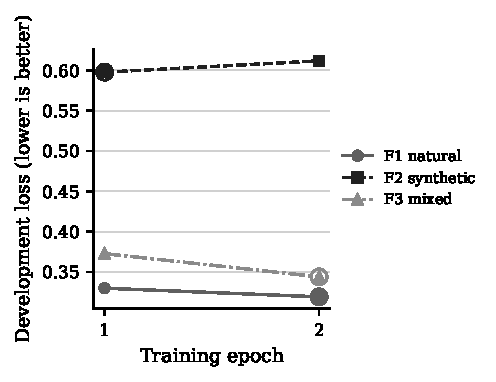
\includegraphics[width=\columnwidth]{figures/checkpoint_dev_loss.pdf}
\caption{Development assistant-token cross-entropy across the two original
training epochs. Lower is better; an open ring marks the checkpoint selected
by the frozen common-development rule. These are selection losses, not final
test scores.}
\label{fig:checkpoint-loss}
\end{figure}

\subsection{Implementation and hardware}

All primary F1--F3 training and B1/B2/F1--F3 final inference use Tesla P100
GPUs with the recorded 4-bit runtime.  The separate post-hoc seed cohort trains
on A100s and evaluates uniformly on RTX 3090s; the matched behavioral
diagnostics use a P100.  Exact package, device, revision, and artifact
identities are recorded once in the public audit and repository rather than
repeated throughout the paper.

\section{Evaluation and Statistical Analysis}

All systems use greedy decoding, no temperature argument, at most 32 new
tokens, and seed 3407.  We retain raw responses before applying a conservative
parser.  Empty outputs, parsing failures, and suspicious multi-token outputs
are recorded rather than repaired.

For the pre-specified F3--F2 comparison, we report the difference in
exact-match accuracy,
an exact two-sided McNemar test, and a deterministic 10,000-sample paired
bootstrap percentile interval with seed 3407.  Both systems are aligned by
the 511 frozen record identifiers.  The interval is conditional on the single
training seed and excludes retraining variance.  Comparisons involving B1, B2,
or F1 were executed or consolidated at different stages and are secondary.
Their intervals and tests are descriptive rather than a simultaneous
five-arm family.

This staging reflects the actual experimental timeline.  F1 was trained and
evaluated before the Tibyan-derived F2/F3 comparison was designed; the frozen
one-access policy ruled out rerunning it merely to make a simultaneous table.
F2 and F3 were then evaluated together as the primary matched contrast.  B1
and B2 were added later to answer a separate prompt-only question and were
frozen before their own test access.  Consequently, only F3--F2 is treated as
the primary simultaneous comparison.

We additionally report a post-hoc training-seed robustness cohort.  Five
independently trained F2/F3 replicas use seeds 3407--3411, the frozen training
recipe, and the same checkpoint rule.  All ten selected adapters are evaluated
from record zero on one uniform hardware path.  The seed-3407 replica does not
reuse either original primary adapter.  This cohort
was run after the primary result and is therefore robustness evidence rather
than a second pre-specified analysis.

Both epoch checkpoints are retained for every replica.  In a further post-hoc
sensitivity, we reuse the selected-checkpoint predictions and evaluate only
the other checkpoint, then compare all arms at fixed epoch 1, fixed epoch 2,
and the frozen dev-selected policy.  This isolates whether selection on the
common natural development view determines the direction of the result.

\section{Results}

\begin{table}[t]
\centering
\small
\begin{tabular}{llrr}
\toprule
System & Setting & Correct & EM (\%) \\
\midrule
B1 & five-shot & 89 & 17.42 \\
B2 & expert-style & 108 & 21.14 \\
\midrule
F1 & natural-only & 145 & 28.38 \\
F2 & synthetic-only & 105 & 20.55 \\
F3 & 50:50 mixed & \textbf{162} & \textbf{31.70} \\
\bottomrule
\end{tabular}
\caption{Exact-match accuracy (EM) on 511 highlighted-token Nahw-Passage
records. Prompt baselines are untouched; F1--F3 are equal-record QLoRA arms.}
\label{tab:main-results}
\end{table}

\begin{figure*}[t]
\centering
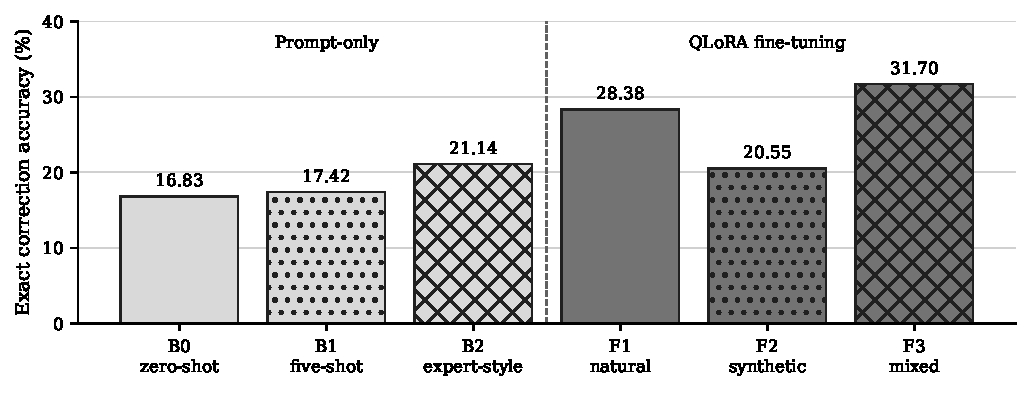
\includegraphics[width=0.82\textwidth]{figures/system_accuracy.pdf}
\caption{Final exact-match accuracy.  Bar patterns distinguish protocols,
not uncertainty. Confirmatory uncertainty is reported for the paired
F3--F2 difference rather than as independent binomial error bars.}
\label{fig:accuracy}
\end{figure*}

Table~\ref{tab:main-results} and Figure~\ref{fig:accuracy} show the final
results.  F3 obtains 162/511 exact matches (31.70\%), compared with 105/511
(20.55\%) for F2.  F3 corrects 89 records missed by F2, whereas F2 corrects 32
missed by F3.  The primary paired difference is 11.15 points, with a 95\%
interval of 7.05--15.26 points and exact McNemar
$p=2.15\times10^{-7}$.  This supports mixed supervision over
synthetic-only supervision under the frozen protocol.

\begin{table}[t]
\centering
\small
\begin{tabular}{lrr}
\toprule
Comparison & Difference & 95\% interval \\
\midrule
F3 $-$ F2 & +11.15 & [7.05, 15.26] \\
F1 $-$ F2 & +7.83 & [3.13, 12.52] \\
F3 $-$ F1 & +3.33 & [$-0.39$, 7.05] \\
F3 $-$ B2 & +10.57 & [6.65, 14.48] \\
F1 $-$ B2 & +7.24 & [3.33, 10.96] \\
\bottomrule
\end{tabular}
\caption{Paired differences in exact-match accuracy, in percentage points.
Only F3--F2 is the
pre-specified primary comparison; the remaining rows are staged secondary
comparisons.}
\label{tab:paired}
\end{table}

F1 reaches 28.38\%, while F2 reaches 20.55\%.  In the staged comparison, F1
exceeds F2 by 7.83 points (interval 3.13--12.52).  F3 is 3.33 points above F1,
but its interval ($-0.39$ to 7.05) includes zero; we therefore do not claim
that mixed supervision is better than natural-only supervision.

Prompt design matters within the displayed untouched-model baselines: B2
exceeds B1 by 3.72 points (interval 0.78--6.65).  F1 and F3 exceed B2 in staged
comparisons.  F2 and B2 differ by only $-0.59$ points, with an interval
spanning zero.  All arms produce 511 aligned parsed predictions with no empty
output or parsing failure.  Suspicious or multi-token outputs number 2 for F1,
20 for F2, 2 for F3, and 6 for B2; they are retained unchanged when scoring.
A post-hoc sensitivity takes the first whitespace-delimited token only for
already flagged outputs and applies the rule symmetrically.  It rescues 0/20
F2 outputs and 0/2 F3 outputs, leaving both scores and the 11.15-point gap
unchanged.  Format compliance therefore explains none of the primary
difference under this sensitivity; the frozen parser remains primary.

\begin{table}[t]
\centering
\scriptsize
\setlength{\tabcolsep}{3pt}
\begin{tabular}{lrrr}
\toprule
Training seed & F2 & F3 & F3 $-$ F2 \\
\midrule
3407-A100 & 20.55 & 33.07 & +12.52 \\
3408 & 21.92 & 31.51 & +9.59 \\
3409 & 21.72 & 30.33 & +8.61 \\
3410 & 22.50 & 33.07 & +10.57 \\
3411 & 21.72 & 31.90 & +10.18 \\
\midrule
Mean (SD) & 21.68 (0.71) & 31.98 (1.15) & +10.29 (1.45) \\
\bottomrule
\end{tabular}
\caption{Post-hoc five-seed robustness cohort. Values are exact-match
accuracy percentages; SD is the sample standard deviation across seeds. All
rows are independent retrains evaluated on one uniform hardware path;
``3407-A100'' is not the original primary run.}
\label{tab:multiseed}
\end{table}

Table~\ref{tab:multiseed} directly addresses training-seed sensitivity.  F3
exceeds F2 in all five seeds; the paired difference ranges from 8.61 to 12.52
points.  The mean difference of 10.29 points (SD 1.45) is close to the
11.15-point primary estimate.  Because this cohort is post-hoc and uses a
different but internally uniform hardware path, it supports robustness of the
direction and magnitude without replacing the primary analysis.  On seed
3407, the independent A100/RTX-3090 path gives F3 169/511 (33.07\%), seven
more exact matches than the original P100 run's 162/511 (31.70\%); F2 happens
to give 105/511 on both paths.  We verified these counts against the frozen
aggregate audits.  Cross-platform bitwise determinism was neither required nor
achieved, so this row is a replication rather than a reproduction of the
original adapter.

\begin{table}[t]
\centering
\small
\begin{tabular}{lrrr}
\toprule
Checkpoint policy & F2 & F3 & F3 $-$ F2 \\
\midrule
Fixed epoch 1 & 21.68 & 27.79 & +6.11 \\
Fixed epoch 2 & 25.40 & 31.98 & +6.58 \\
Dev-selected & 21.68 & 31.98 & +10.29 \\
\bottomrule
\end{tabular}
\caption{Post-hoc five-seed checkpoint sensitivity. Values are mean exact-
match percentages. F3 exceeds F2 in every seed under both fixed policies.}
\label{tab:checkpoints}
\end{table}

Table~\ref{tab:checkpoints} shows that the mixed-over-synthetic direction is
not created by the natural-development selection rule: the mean gap remains
6.11 points at fixed epoch 1 and 6.58 points at fixed epoch 2.  However, the
rule selects epoch 1 for every F2 replica and epoch 2 for every F3 replica,
expanding the dev-selected gap to 10.29 points.  The selection policy therefore
affects effect magnitude even though both matched policies preserve its sign.

\section{Auxiliary Behavioral Diagnostics}

Before the F1 diagnostic was run, we froze two matched checks and regenerated
a fresh untouched-base control (\textbf{B0}) beside F1 within one run.
This is distinct from the excluded historical T4 Nahw evaluation.  First, on
154 corrected QALB-2015 L2 development sentences, each record designates one
Arabic-script token already present in the corrected target.  F1 leaves the
designated token unchanged in 78/154 cases (50.65\%), compared with 43/154
(27.92\%) for B0.  The paired difference is 22.73 points (95\% interval
12.34--33.12).  This indicates less overcorrection on this selected
development diagnostic, not on arbitrary correct Arabic.

Second, we evaluate a balanced 1,000-question subset spanning all 40
ArabicMMLU tasks \citep{koto-etal-2024-arabicmmlu}.  B0 scores 53.7\% and F1
53.1\%; the $-0.6$-point difference has a stratified paired-bootstrap interval
of $-3.2$ to $+1.9$ points.  This does not establish non-inferiority or general
capability retention.

We subsequently apply the same frozen diagnostics to the original F2 and F3
adapters in one matched run.  F2 leaves the designated correct token
unchanged in 97/154 cases (62.99\%), whereas F3 does so in 35/154 (22.73\%).
The primary F3--F2 difference is $-40.26$ points (95\% interval $-49.35$ to
$-31.17$; exact McNemar $p<10^{-13}$).  On ArabicMMLU, F2 scores 48.7\% and
F3 54.0\%, a primary difference of $+5.30$ points (40-task stratified interval
$+3.10$ to $+7.60$; $p<10^{-5}$).  Thus synthetic-only supervision resists
overcorrection better on this narrow diagnostic, while mixed supervision
retains substantially more measured capability.  B0/F1 comparisons remain
staged references, and we make no broad safety claim.

\section{Discussion}

The primary result shows that synthetic examples are not interchangeable with
natural supervision at fixed record count.  Adding natural data to the
synthetic view closes a large performance deficit and does so across all five
post-hoc seeds.  This is consistent with natural examples better matching the
task interface or correction distribution while synthetic examples provide
complementary coverage.  The experiment cannot distinguish those mechanisms:
QALB and Tibyan differ in record length, token count, domain, error
distribution, and correction quality.

The F1--F2 secondary result also favors natural supervision, while the F3--F1
interval includes zero.  The appropriate conclusion is therefore not that
mixing is universally optimal.  Rather, mixing substantially repairs the
deficit of the synthetic-only view and reaches performance statistically
compatible with the natural-only arm under this test.  Additional models,
sizes, languages, and independently licensed test sets are required to
separate a general mixture effect from a dataset-specific interaction.

The prompt baselines sharpen this interpretation.  A more explicit
expert-style instruction improves the untouched model, but F1 and F3 remain
well above it in secondary comparisons.  Conversely, F2 is statistically
compatible with B2.  Fine-tuning alone is therefore not sufficient;
supervision source remains consequential.

The auxiliary diagnostics add an important qualification: the mixed arm's GEC
advantage does not imply uniformly better behavior.  Relative to F2, F3 trades
substantially higher selected-token overcorrection for higher ArabicMMLU
accuracy.  The two measures cover different behaviors, so neither arm dominates
the other outside the frozen correction test.

\section{Reproducibility and Artifact Boundaries}

We record the immutable base revision, selected-checkpoint identities, data
selection hashes, exact prompt and parser versions, decoding configuration,
package versions, hardware, private prediction hashes, and statistical seed.
Every final aggregate is independently recomputed from aligned private
predictions.  Timeout-safe evaluation persists each row and resumes only after
verifying the exact prefix, avoiding regeneration of completed predictions.

Code, protocols, corpus-free summaries, aggregate statistics, and hashes are
eligible for an anonymized review package.  QALB-derived records, Nahw text,
record-level predictions, raw model responses, logs, checkpoints, and adapters
are not redistributed under the applicable data and artifact restrictions.
The published code lets a licensed custodian recompute every count and paired
statistic from aligned private rows; published hashes establish which exact
inputs, predictions, and checkpoints were audited.  Hashes do not reveal the
rows or permit an unlicensed reviewer to rescore them, so fully independent
end-to-end replication remains limited.  The upstream Tibyan release remains
available under its own license.

\section{Conclusion}

In a frozen equal-record comparison, a 50:50 natural--synthetic mixture
substantially outperforms synthetic-only supervision for Gemma 3 4B Arabic
highlighted-token GEC, and a post-hoc five-seed cohort preserves this direction
in every seed and at both matched epoch checkpoints.  Development selection
amplifies the mean separation but does not create it.  Natural-only supervision also exceeds synthetic-only
supervision in a staged comparison, while mixed supervision is not established
as better than natural-only.  Together with prompt baselines, the results
indicate that data composition---not fine-tuning alone---is a central
experimental variable for open-weight Arabic GEC.

\section{Limitations}

Our evidence is limited to one 4B model, one equal-record training size, and
one principal test set.  Record matching does not equalize tokens, domains, or
error categories.  The primary interval is conditional on seed 3407; the
post-hoc cohort finds a positive paired difference in every seed but uses a
different, internally uniform hardware path.  Although F2 contains more
tokens than F3, token totals do not control length, domain, or source quality.
We do not run QALB test, so our exact-match accuracy is not comparable to
full-sentence M2 scores.

Every trainable arm selects between epoch 1 and epoch 2 using loss on the same
natural QALB development view.  The rule was frozen before test access, but a
natural development distribution could still favor F3 over F2.  In the
post-hoc fixed-epoch sensitivity, F3 remains higher under both matched policies,
but the rule selects F2 epoch 1 and F3 epoch 2 for all five replicas and expands
the mean gap from roughly 6 points to 10.29.  Thus checkpoint selection does
not determine the sign here, but it materially affects the estimated magnitude.

Exact single-reference matching is intentionally strict.  A linguistically
valid alternative receives no credit unless it equals the supplied token.
No qualified linguist reviewed the private predictions, so we provide no
error-type or expert-quality claims.  ARETA-derived aggregate evidence in the
source literature does not substitute for expert labels on our outputs.

F1, F2/F3, and the prompt baselines were executed at different stages, so only
the simultaneously executed F3--F2 contrast is primary.  The earlier F1 and
later prompt-only systems were frozen before their respective test access, but
they cannot retrospectively become one simultaneous experiment.  We exclude
the historical T4 Nahw baseline and all comparisons derived from it.  Hardware
for retained primary, staged, robustness, and diagnostic runs is consolidated
in the experimental setup rather than treated as an experimental variable.

Our exact-hash overlap checks do not detect paraphrases, shared upstream
sources, or unknown pretraining contamination.  The overcorrection diagnostic
uses one designated token from corrected QALB development text and does not
measure sentence-level preservation or all valid alternatives.  ArabicMMLU is
a selected balanced subset rather than a formal non-inferiority design.
Finally, restricted artifacts prevent public release of the full training and
prediction package.

\section{Ethical Considerations}

The work concerns text correction and does not involve participant recruitment
or new human annotation.  We preserve official dataset roles, keep
Nahw-Passage test-only, and do not use QALB test for modeling or evaluation.
QALB-derived material is kept private under its research conditions; Tibyan
attribution and CC BY 4.0 terms are preserved; ArabicMMLU questions remain
private under CC BY-NC 4.0.

Automated correction can encode prescriptive language norms and should not be
used to stigmatize dialectal Arabic or writers.  Our task and claims concern
MSA highlighted-token correction only.  ``Expert-style'' refers solely to a
prompt design, and we make no claim of expert linguistic validation.  Adapters
trained on restricted natural data remain private pending legal,
institutional, and model-license review.

\bibliography{references}

\end{document}
